\M
The \define{Hypergeometric Distribution} occurs in situations like:
\begin{quote}
Suppose we have $N$ balls, of which $k$ are red and $N-k$ are blue. We
draw a sample, without replacement, of $n$ balls. Let $X$ be the number
of red balls drawn in our sample of size $n$. What's the probability
$X=x$?
\end{quote}
We see
\begin{equation}
\Pr(X=x)=\frac{\begin{pmatrix}\mbox{number of different}\\
\mbox{ways to choose}\\
\mbox{$x$ red balls}
\end{pmatrix}
\begin{pmatrix}
\mbox{number of different}\\
\mbox{ways to choose}\\
\mbox{$(n-x)$ blue balls}
\end{pmatrix}}{\begin{pmatrix}\mbox{number of different}\\
\mbox{samples drawn}
  \end{pmatrix}}
\end{equation}

\N{Example}
We have 1000 widgets, of which an unknown number $D$ has defects. A
sample of 100 has 2 with defects. The \define{Maximum Likelihood Estimate}
for $D$ is the number which gives the highest probability for obtaining
the number of defectives observed in a sample. Find that value of $D$.

\N*{Solution:}
So we have $N=1000$ and instead of ``red balls'' we have ``defective
Widgets'' $k=D$. The sample size is $n=100$. What's the value of $D$
that makes the event most probable?

Well, the distribution would be described by
\begin{equation}
\Pr(X=2)=\frac{\binom{D}{2}\binom{1000-D}{100-2}}{\binom{1000}{100}}
\end{equation}
which algebraically reduces to
\begin{equation}
\Pr(X=2)=\frac{D(D-1)}{2}\frac{1}{100\cdot999\cdot(\dots)\cdot(1000-(D-1))}
\frac{900\cdot(\dots)\cdot(902-(D-1))}{1}\cdot100\cdot99.
\end{equation}
We can then write up a small Python program which will write out a table for
values of $D$ and the corresponding probability.
\begin{python}
import math

# Stirling's approximation
def factorial(n):
    x = 1.0*n
    return math.sqrt(2*math.pi*x)*math.pow(x/math.e,x)

# return a*(a+1)*(...)*b
def product(a, b):
    if a>b:
        return product(b,a)
    else:
        result = 1.0
        for k in xrange(a,b+1):
            result = result*k
        return result

# probability X = D
def hypergeometricProbability(X):
    c = 990.0
    return c*(X*(X-1)*0.5) * product(902-X+1,900)/product(1000-X+1,1000)

for D in xrange(19,24):
    v = hypergeometricProbability(D)
    print "D=%d, Pr(X=2) = %f\n" % (D, v)
\end{python}
A small snippet reveals:
\begin{Verbatim}[fontsize=\footnotesize]
D=19, Pr(X=2) = 0.028804
D=20, Pr(X=2) = 0.028807
D=21, Pr(X=2) = 0.028655
D=22, Pr(X=2) = 0.028366
D=23, Pr(X=2) = 0.027954
\end{Verbatim}
which implies $D=20$ is the value which has the most probable
outcome. 
\N{Example}
On an Island, 50 moose are captured and tagged. Six months later, 200
moose are captured, of which 8 are tagged. Estimate the number of moose
on the Island.

\N*{Solution:}
So, this is a hypergeometric distribution, where the ``red balls'' are
the tagged moose, we have a sample of 200 without replacement, and 8 of
them are tagged. So we are trying to maximize the function
\begin{equation}
h(N,50,200,8)=\frac{\binom{50}{8}\binom{N-50}{200-8}}{\binom{N}{200}}
\end{equation}
by picking some $N$. After some algebra, we can rewrite this as
\begin{equation}
\begin{split}
h(N,50,200,8)&=\frac{50!}{42!}\frac{1}{8!}\frac{200!}{192!}\frac{(N-50)!}{N!}\frac{(N-200)!}{(N-242)!}\\
&=C\frac{(N-50)!}{N!}\frac{(N-200)!}{(N-242)!}
\end{split}
\end{equation}
where $C=1192725059258223539848800000$. 
We have $N\geq242$. We write up a small program, listed below, to write
out a table of probabilities. It's maximized when $N=1250$.

Graphically, the ``most likely'' situation may be visualized as the
point which maximizes the probability. For our particular problem, we
plot the probability and place a red dot where the probability maximized
(``most likely''): 

\begin{center}
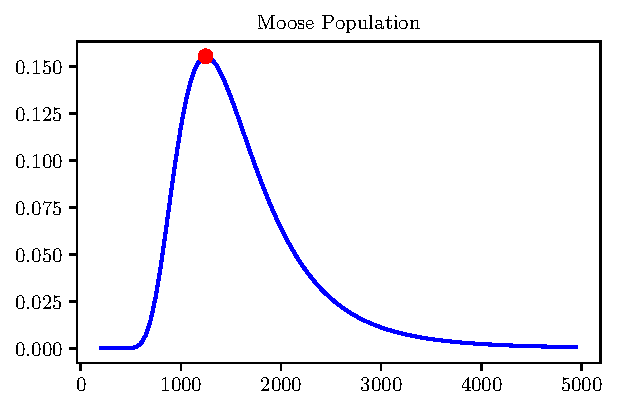
\includegraphics{img/moose.pdf}
\end{center}


\begin{python}
# using the product() function previously defined
def moosePopulation(N):
    c = 1192725059258223539848800000.0
    return c * product(N-200,N-241)/product(N-49,N)

for N in xrange(1242, 1261):
    v = moosePopulation(N)
    print "N=%d, h(N,50,200,8) = %.20f" % (N,v)
\end{python}

\N{Example}
Suppose that in a bushel of 550 apples there are 2\% rotten ones. What
is the probability that a random sample of 25 apples contains two
rotten apples? Hint: Hypergeometric distribution.

\N*{Solution:}
So, we have $N=550$ apples, of which $k=11$ are rotten. So we pick a
sample $n=25$. What's the probability $x=2$ are rotten? It's given by
\begin{equation}
\Pr(\mbox{2 rotten})=\frac{\binom{11}{2}\binom{539}{23}}{\binom{550}{25}}
\end{equation}
We can compute this by hand, finding
\begin{equation}
\begin{split}
\Pr(\mbox{2 rotten})
&=\frac{599494391824595575}{8092091399320955412}\\
&\approx 0.074083986
\end{split}
\end{equation}
so the probability is roughly $7.4\%$.
